\pdfminorversion=4
%\documentclass[handout,13pt,aspectratio=169]{beamer}
\documentclass[13pt,aspectratio=43]{beamer}
\usepackage[utf8]{inputenc}

\usetheme{metropolis}

\usepackage{appendixnumberbeamer}
% \usepackage[italian]{babel}
% \usepackage[english]{babel}
\title{
	Performance analysis for TCP BBR in Mininet
}

\date{\today}
\author{Massimo Girondi}
%\titlegraphic{\center\includegraphics[height=2cm]{unitn_trasp.pdf}\\
%\footnotesize Dipartimento di Informatica e Scienza dell'Informazione}
%\metroset{background=dark}


\begin{document}

\maketitle
%\begin{frame}{Table of contents}
%  \setbeamertemplate{section in toc}[sections numbered]
%  \tableofcontents[hideallsubsections]
%\end{frame}

\begin{frame}{TCP BBR}
	\begin{itemize}
		\item Developed by Google
		\item OpenSource
		\item blah blah blah
	\end{itemize}
\end{frame}

\begin{frame}{Test setup}
	\begin{itemize}
		\item Mininet 2.3 on Debian 9
		\item Virtual machine running on VirtualBox
		\item Provisioned through Vagrant 
	\end{itemize}
\end{frame}
\begin{frame}{Topology}
  \begin{figure}
	  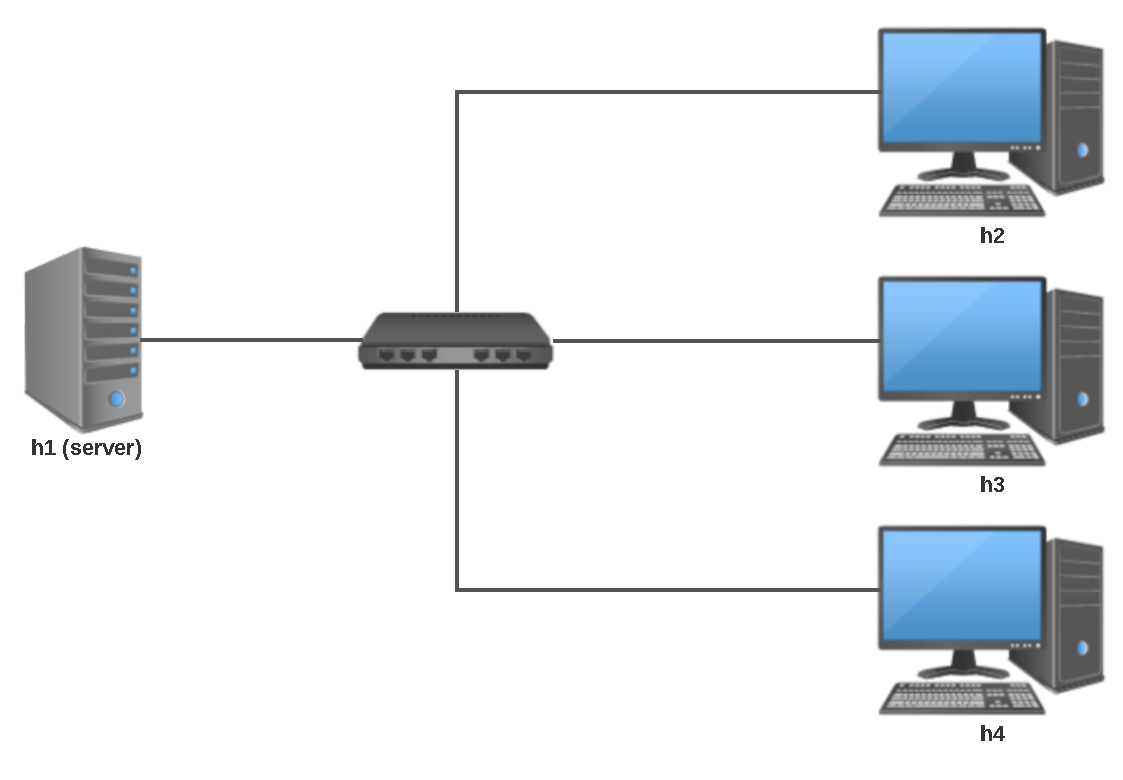
\includegraphics[width=\textwidth,height=\textheight,keepaspectratio]{network.pdf}
  \end{figure}
\end{frame}

\begin{frame}{20 seconds Iperf test: description}
	\begin{itemize}
		\item \texttt{h1} as server
		\item \texttt{h2} as client
		\item Client options: \texttt{-f k -c IP -t 20 }
			\begin{itemize}
				\item[-f k] kbps as output format
				\item[-t 20] Run for 20 seconds
			\end{itemize}
	\end{itemize}
\end{frame}

\begin{frame}{20 seconds Iperf test: results [1/2]}
  \begin{figure}
	  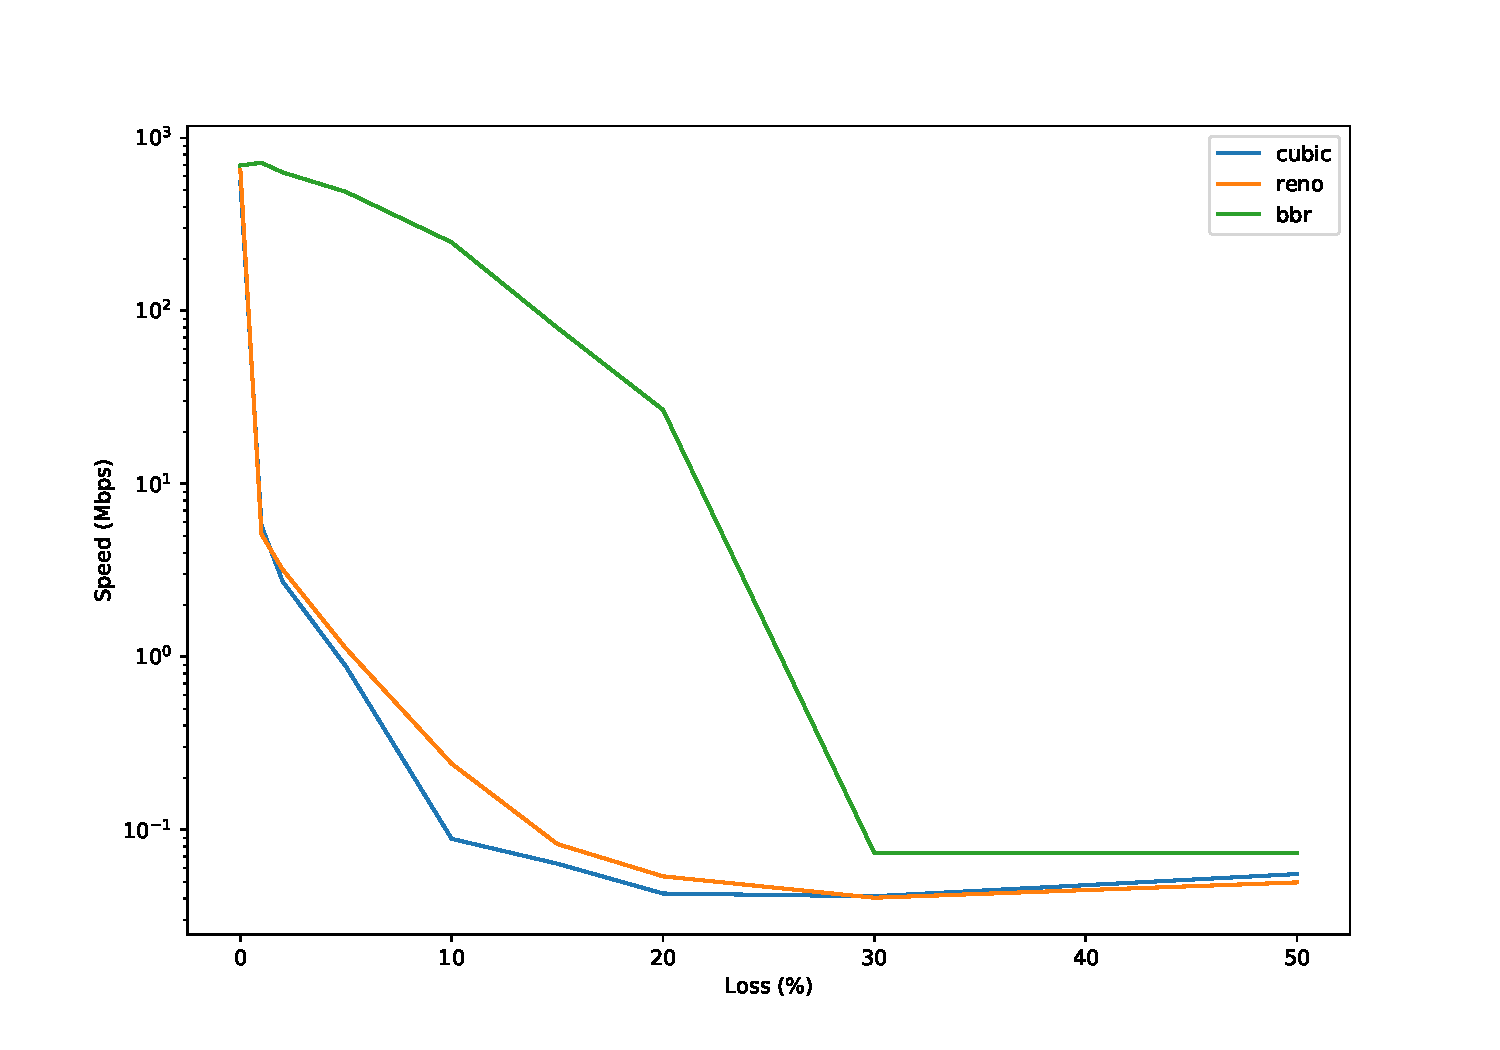
\includegraphics[width=\textwidth,height=\textheight,keepaspectratio]{../iperf_test/plot_log.pdf}
  \end{figure}
\end{frame}

\begin{frame}{20 seconds Iperf test: results [2/2]}
  \begin{figure}
	  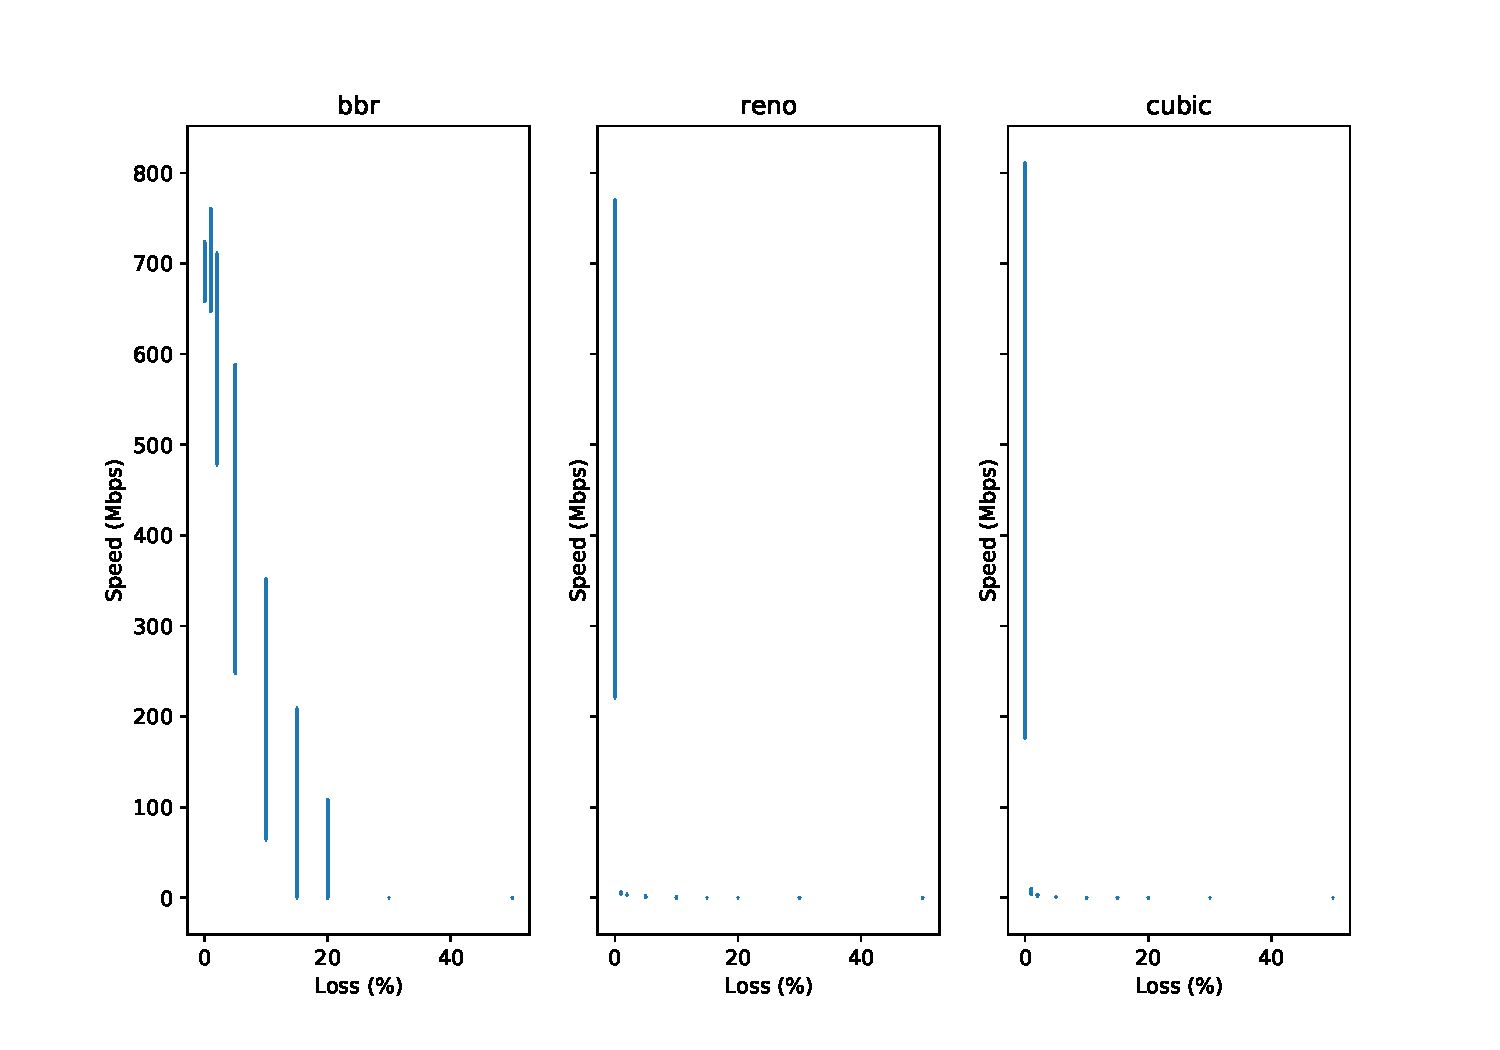
\includegraphics[width=\textwidth,height=\textheight,keepaspectratio]{../iperf_test/violinplot.pdf}
  \end{figure}
\end{frame}


\begin{frame}{Complex web page simulation: description}
	\begin{itemize}
		\item \texttt{h1} as server
		\item \texttt{h2} as client
		\item \texttt{nginx} as server since Python's \texttt{SimpleHTTPServer} is too slow
		\item \texttt{wget -r} as client, simulating the web page browsing
		\item \texttt{bbc.co.uk} index page as an example: elements has same size but random data
		\item 72 elements with a total size of 2.902 MB
		\item Speed is obviously slower than a single big file download
		\item Elements included as images into a simple HTML file
	\end{itemize}
\end{frame}

\begin{frame}{Complex web page simulation: page structure}
  \begin{figure}
	  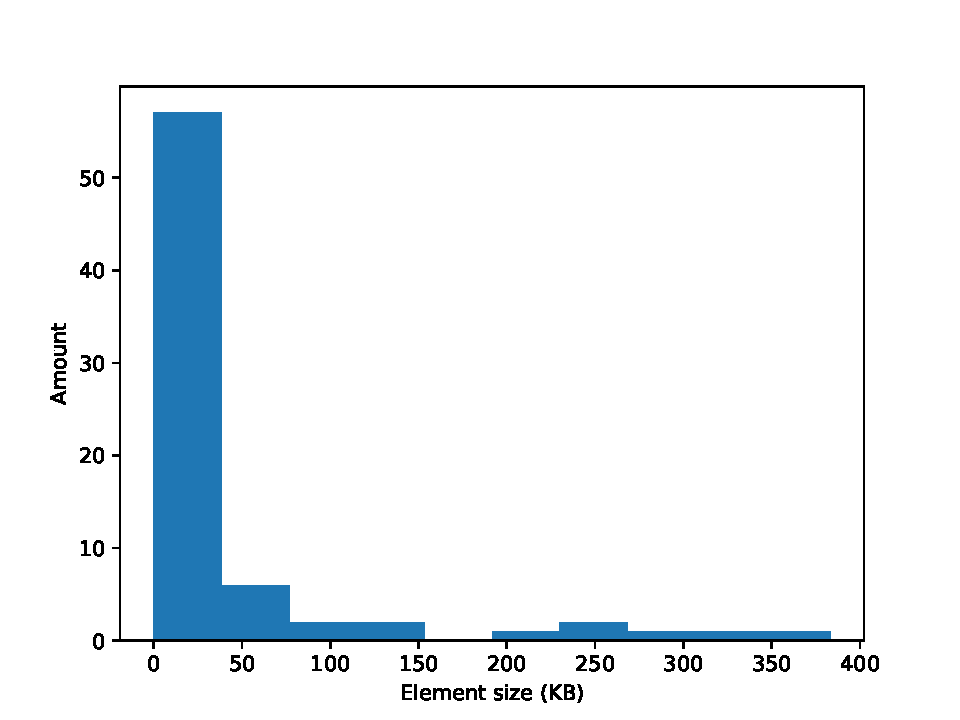
\includegraphics[width=\textwidth,height=\textheight,keepaspectratio]{../http_test/page_stat.pdf}
  \end{figure}

\end{frame}



\begin{frame}{Complex web page simulation: results [1/2]}
  \begin{figure}
	  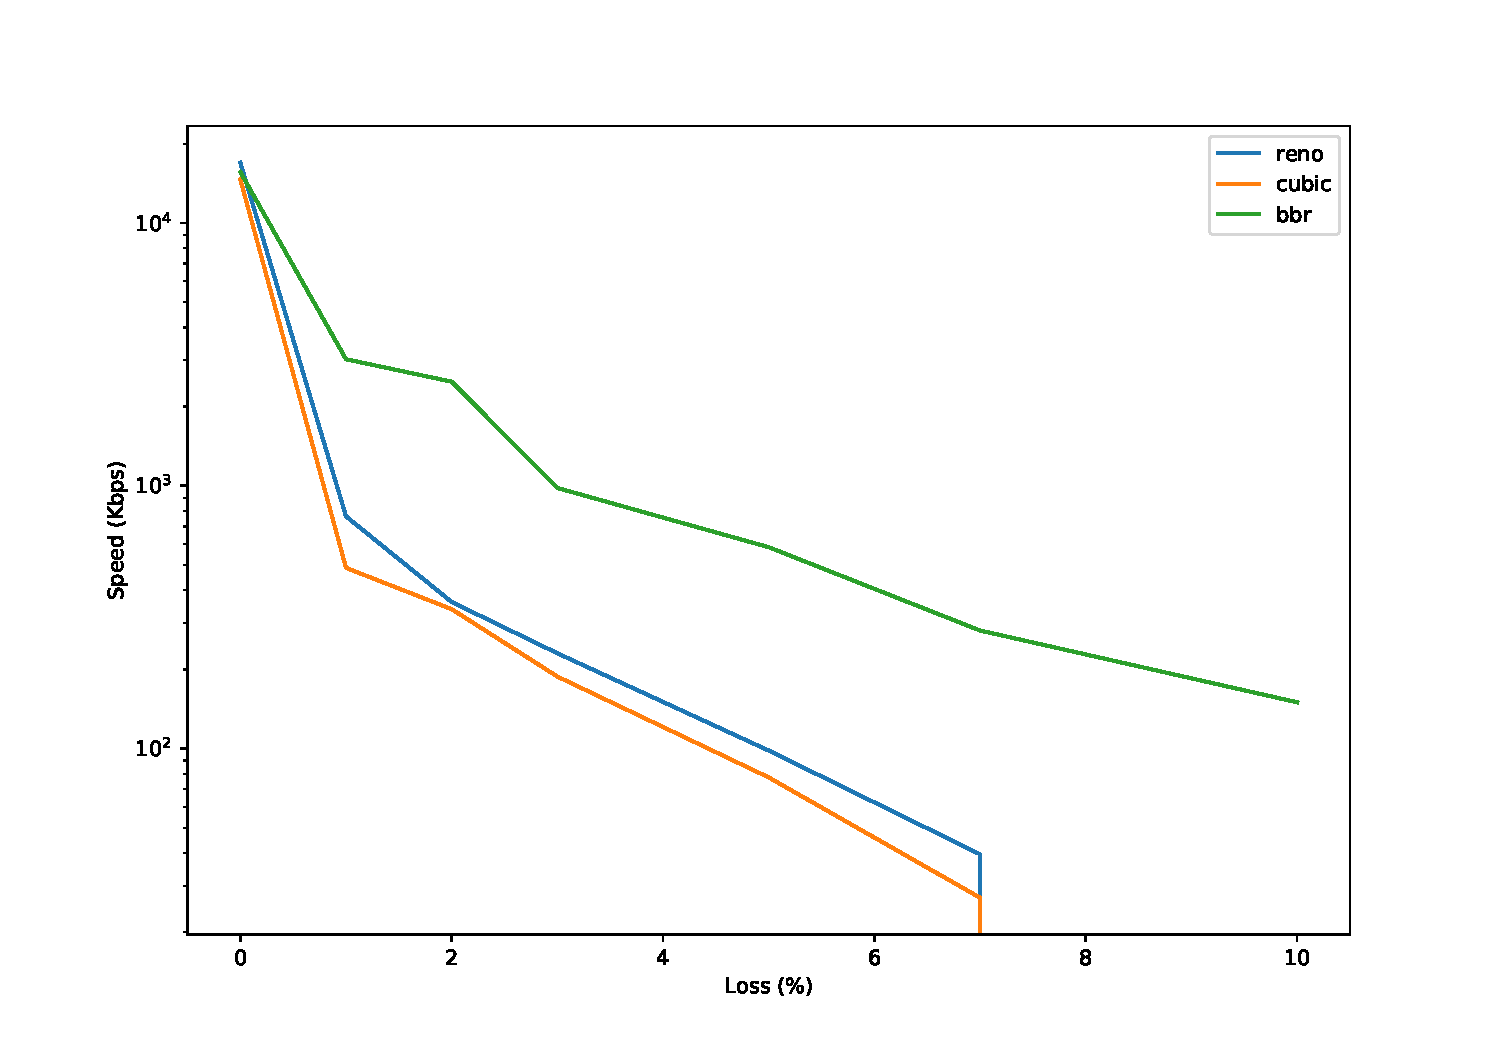
\includegraphics[width=\textwidth,height=\textheight,keepaspectratio]{../http_test/plot_log.pdf}
  \end{figure}
\end{frame}

\begin{frame}{Complex web page simulation: results [2/2]}
  \begin{figure}
	  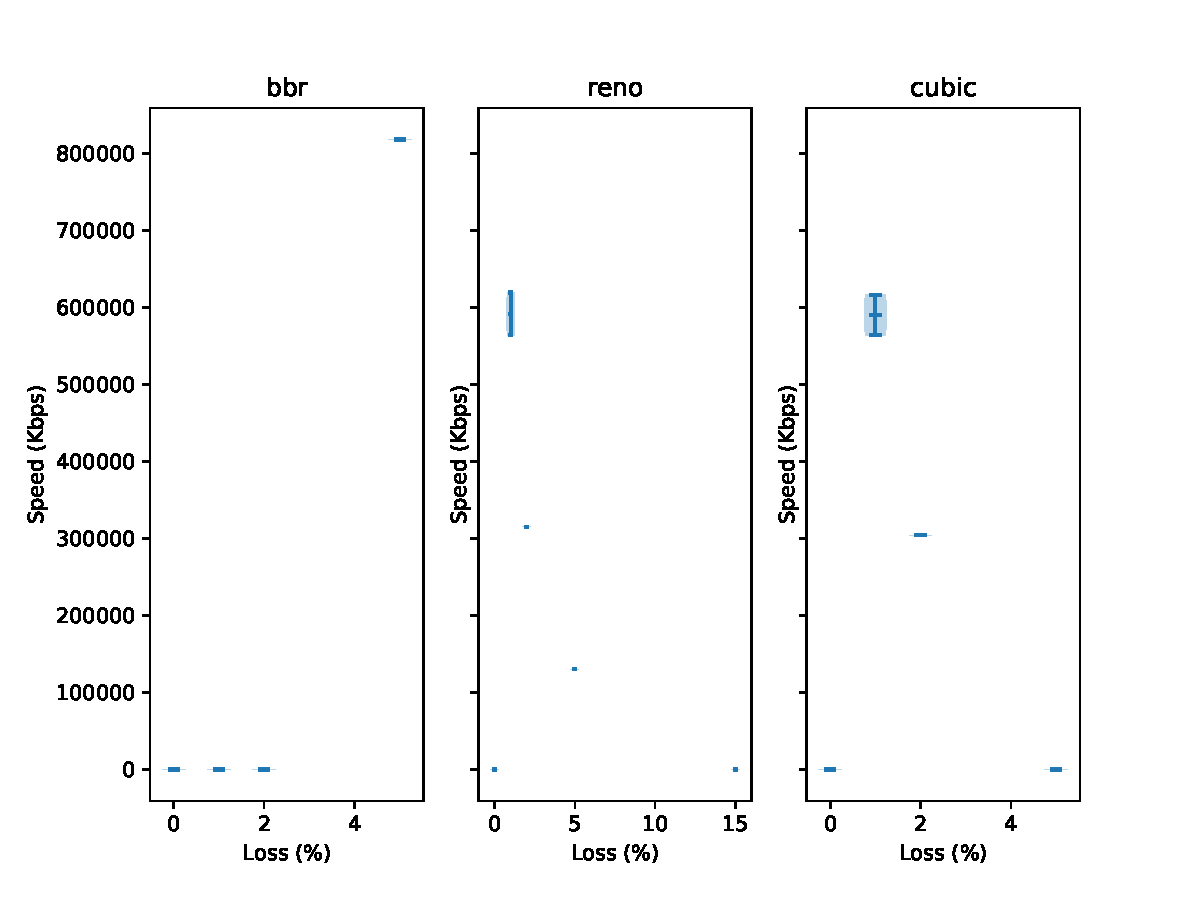
\includegraphics[width=\textwidth,height=\textheight,keepaspectratio]{../http_test/violinplot.pdf}
  \end{figure}
\end{frame}



\begin{frame}{Topology}
\end{frame}



\end{document}
